\documentclass[tikz,border=5mm]{standalone}
\pagecolor{gray}
\begin{document}
	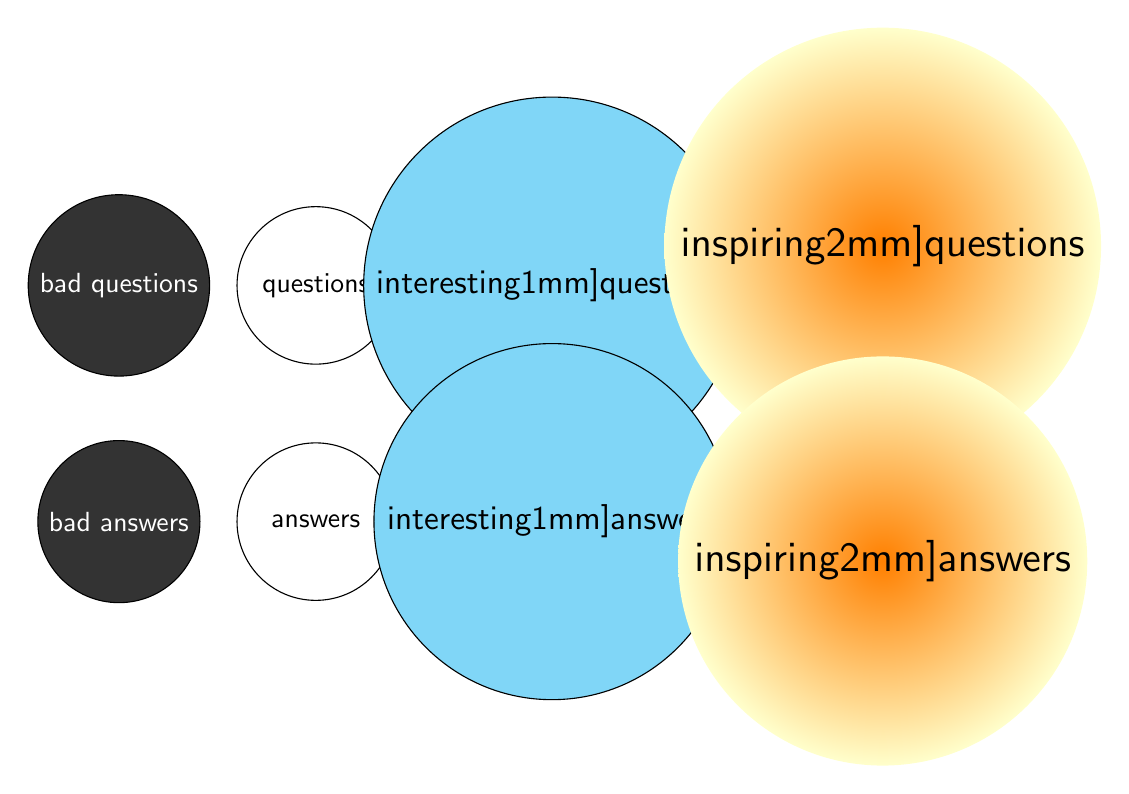
\begin{tikzpicture}[every node/.style={circle,draw,font=\sffamily,align=center}]
		\path[nodes={minimum size=2cm,fill=black!80,text=white}] (-2.5,0)
		+(90:1.5) node{bad questions}
		+(-90:1.5) node{bad answers};
		\path[nodes={minimum size=2cm,fill=white}] (0,0)
		+(90:1.5) node{questions}
		+(-90:1.5) node{answers};
		\path[nodes={minimum size=2.5cm,scale=1.2,fill=cyan!50}] (3,0)
		+(90:1.5) node{interesting\[1mm]questions}
		+(-90:1.5) node{interesting\[1mm]answers};
		\path[nodes={draw=none,inner color=orange,outer color=yellow!20,scale=1.5,minimum size=3cm}] (7.2,0)
		+(90:2) node{inspiring\[2mm]questions}
		+(-90:2) node{inspiring\[2mm]answers};
	\end{tikzpicture}
\end{document}